\section{Лекция 3. Теорема Пикара и метод последовательных приближений}
\noeqref{eq:l3_cauchy_eq, eq:l3_cauchy_ic, eq:l3_lipschitz_y, eq:l3_riccati_ex}
\noeqref{eq:l3_int_eq, eq:l3_picard_seq}

\begin{flushright}
    21.09.26
\end{flushright}

\subsection{Теорема Пикара о существовании и единственности}

Рассмотрим задачу Коши для дифференциального уравнения 1-го порядка:
\begin{align}
    y' &= f(x, y), \tag{1} \label{eq:l3_cauchy_eq} \\
    y(x_0) &= y_0. \tag{2} \label{eq:l3_cauchy_ic}
\end{align}

Обобщим введённое в Лекции 2 понятие условия Липшица на случай функции двух
переменных $f(x, y)$ в замкнутом прямоугольнике
\[
    \Pi = \left\{ (x, y) \in \R^2 : \abs{x - x_0} \le a, \;
    \abs{y - y_0} \le b \right\}, \quad a, b > 0.
\]

\begin{definition}
    Функция $f(x, y)$ удовлетворяет \textdef{условию Липшица по переменной $y$}
    в прямоугольнике $\Pi$, если существует константа $L > 0$ такая, что для
    любых двух точек $(x, y_1), (x, y_2) \in \Pi$ с одинаковой абсциссой $x$
    выполняется неравенство:
    \begin{equation} \label{eq:l3_lipschitz_y}
        \abs{f(x, y_2) - f(x, y_1)} \le L \abs{y_2 - y_1}. \tag{3}
    \end{equation}
\end{definition}

\begin{remark}
    Аналогично одномерному случаю из Лекции 2 (по теореме Лагранжа), если
    функция $f(x, y)$ имеет в замкнутом прямоугольнике $\Pi$ непрерывную
    частную производную $\dfrac{\partial f}{\partial y} \in C(\Pi)$, то она
    гарантированно удовлетворяет условию Липшица по $y$ в $\Pi$ с константой
    $L = \max_{(x, y) \in \Pi} \abs{\dfrac{\partial f}{\partial y}(x, y)}$.
\end{remark}

\begin{theorem}[\textbf{Теорема Пикара}]
    Пусть функция $f(x, y)$ непрерывна в замкнутом прямоугольнике $\Pi$, то
    есть $f \in C(\Pi)$, и удовлетворяет в $\Pi$ условию Липшица
    \eqref{eq:l3_lipschitz_y} по переменной $y$.

    Тогда на отрезке $[x_0 - h, x_0 + h]$, где
    \[
        h = \min\left(a, \frac{b}{M}\right), \quad
        M = \max_{(x, y) \in \Pi} \abs{f(x, y)},
    \]
    существует \textdef{единственное} решение $y = y(x)$ задачи Коши
    \eqref{eq:l3_cauchy_eq}, \eqref{eq:l3_cauchy_ic}.
\end{theorem}

\begin{figure}[H]
    \centering
    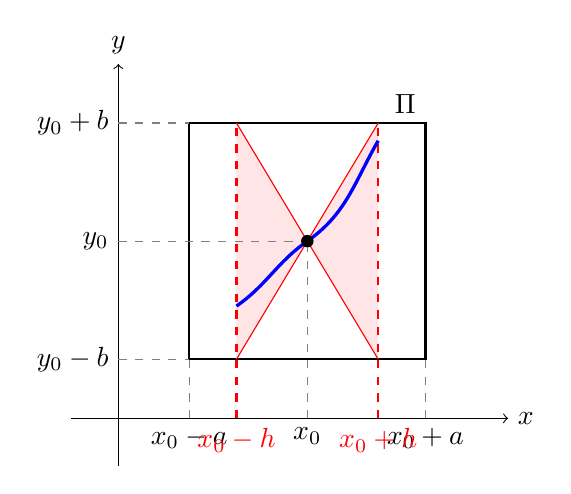
\begin{tikzpicture}[scale=1.5]
        % Оси координат
        \draw[->] (-0.4, 0) -- (3.3, 0) node[right] {$x$};
        \draw[->] (0, -0.4) -- (0, 3.0) node[above] {$y$};

        % Центр прямоугольника
        \def\xO{1.6}
        \def\yO{1.5}
        \def\h{0.6}

        % Прямоугольник \Pi (a = 1, b = 1)
        \draw[thick] (\xO - 1, \yO - 1) rectangle (\xO + 1, \yO + 1);
        \node[above left] at (\xO + 1, \yO + 1) {$\Pi$};

        % Проекции границ прямоугольника
        \draw[dashed, gray] (\xO - 1, 0) node[below, black] {$x_0 - a$}
            -- (\xO - 1, \yO - 1);
        \draw[dashed, gray] (\xO + 1, 0) node[below, black] {$x_0 + a$}
            -- (\xO + 1, \yO - 1);
        \draw[dashed, gray] (0, \yO - 1) node[left, black] {$y_0 - b$}
            -- (\xO - 1, \yO - 1);
        \draw[dashed, gray] (0, \yO + 1) node[left, black] {$y_0 + b$}
            -- (\xO - 1, \yO + 1);

        % Конус предельного наклона y = y_0 \pm M(x - x_0)
        \fill[red!10] (\xO, \yO) -- (\xO + \h, \yO + 1)
            -- (\xO + \h, \yO - 1) -- cycle;
        \fill[red!10] (\xO, \yO) -- (\xO - \h, \yO + 1)
            -- (\xO - \h, \yO - 1) -- cycle;
        \draw[red, thin] (\xO - \h, \yO - 1) -- (\xO + \h, \yO + 1);
        \draw[red, thin] (\xO - \h, \yO + 1) -- (\xO + \h, \yO - 1);

        % Границы отрезка [x_0 - h, x_0 + h]
        \draw[dashed, red, thick] (\xO - \h, 0) node[below] {$x_0 - h$}
            -- (\xO - \h, \yO + 1);
        \draw[dashed, red, thick] (\xO + \h, 0) node[below] {$x_0 + h$}
            -- (\xO + \h, \yO + 1);

        % Проекции центра
        \draw[dashed, gray] (\xO, 0) node[below, black] {$x_0$} -- (\xO, \yO);
        \draw[dashed, gray] (0, \yO) node[left, black] {$y_0$} -- (\xO, \yO);

        % Интегральная кривая
        \draw[blue, very thick] (\xO - \h, \yO - 0.55)
            to[out=35, in=215] (\xO, \yO)
            to[out=35, in=240] (\xO + \h, \yO + 0.85);
        \fill[black] (\xO, \yO) circle (1.5pt);
    \end{tikzpicture}
    \caption{Геометрический смысл выбора $h = \min(a, b/M)$: поскольку наклон
    решения по модулю не превосходит $M$, на отрезке $[x_0 - h, x_0 + h]$
    интегральная кривая гарантированно не покидает прямоугольник $\Pi$ через
    верхнюю или нижнюю крышку $y = y_0 \pm b$.}
\end{figure}

\begin{remark} ~
    \begin{enumerate}
        \item Для самого факта \textit{существования} решения достаточно лишь
        непрерывности $f \in C(\Pi)$ (\textbf{теорема Пеано}). Условие Липшица
        требуется именно для гарантии \textit{единственности}.
        \item Теорема Пикара формулирует достаточное (но не необходимое)
        условие единственности: условие Липшица можно ослабить (например, в
        критерии Осгуда или критерии для автономных ОДУ в Лекции 4).
        \item Теорема Пикара носит \textbf{локальный характер}: она
        гарантирует существование и единственность решения лишь на малом
        отрезке $[x_0 - h, x_0 + h]$, даже если правая часть уравнения
        бесконечно гладкая на всей плоскости.
    \end{enumerate}
\end{remark}

\begin{example}
    Приведём пример уравнения с бесконечно дифференцируемой на всей плоскости
    правой частью $f(x, y) \in C^\infty(\R^2)$, решения которого разрушаются
    за конечное время и не могут быть продолжены на всю числовую прямую $\R$:
    \begin{equation} \label{eq:l3_riccati_ex}
        y' = y^2 - 2y + 1 \iff y' = (y - 1)^2. \tag{4}
    \end{equation}

    \begin{proof}[Решение]~\\
        \begin{quote}
            Приравнивая правую часть к нулю, находим единственное стационарное
            решение $y(x) \equiv 1$, которое определено на всём $\R$.

            При $y \neq 1$ разделяем переменные и интегрируем:
            \[
                \frac{dy}{(y - 1)^2} = dx \implies
                \int (y - 1)^{-2} \, dy = \int dx,
            \]
            \[
                -\frac{1}{y - 1} = x + C \implies
                y(x) = 1 - \frac{1}{x + C}.
            \]
            Каждая такая интегральная кривая имеет вертикальную асимптоту при
            $x = -C$ и уходит на бесконечность за конечное изменение аргумента
            $x$. Поэтому любое нестационарное решение задачи Коши существует
            лишь на одном из открытых лучей $(-\infty, -C)$ или $(-C, +\infty)$.
        \end{quote}
    \end{proof}
\end{example}

\begin{figure}[H]
    \centering
    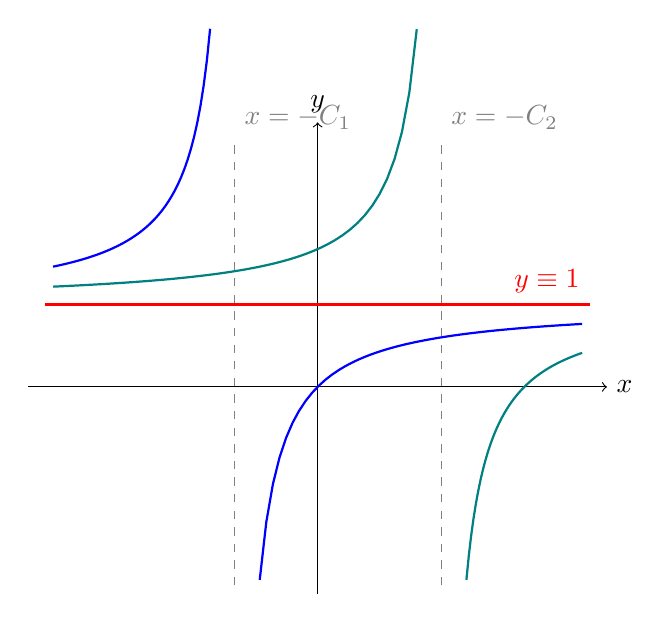
\begin{tikzpicture}[scale=1.05]
        % Оси координат
        \draw[->] (-3.5, 0) -- (3.5, 0) node[right] {$x$};
        \draw[->] (0, -2.5) -- (0, 3.2) node[above] {$y$};

        % Стационарное решение y = 1
        \draw[red, very thick] (-3.3, 1) -- (3.3, 1)
            node[above left] {$y \equiv 1$};

        % Гипербола 1 (C = 1, асимптота x = -1)
        \draw[dashed, gray] (-1, -2.4) -- (-1, 3.0)
            node[above right] {$x = -C_1$};
        \draw[blue, thick, domain=-3.2:-1.3, samples=50]
            plot (\x, {1 - 1/(\x + 1)});
        \draw[blue, thick, domain=-0.7:3.2, samples=50]
            plot (\x, {1 - 1/(\x + 1)});

        % Гипербола 2 (C = -1.5, асимптота x = 1.5)
        \draw[dashed, gray] (1.5, -2.4) -- (1.5, 3.0)
            node[above right] {$x = -C_2$};
        \draw[teal, thick, domain=-3.2:1.2, samples=50]
            plot (\x, {1 - 1/(\x - 1.5)});
        \draw[teal, thick, domain=1.8:3.2, samples=50]
            plot (\x, {1 - 1/(\x - 1.5)});
    \end{tikzpicture}
    \caption{Интегральные кривые уравнения $y' = (y - 1)^2$: стационарная
    прямая $y \equiv 1$ и гиперболы с вертикальными асимптотами $x = -C$.}
\end{figure}

\subsection{Схема доказательства теоремы Пикара}

\textbf{Этап 1. Переход к эквивалентному интегральному уравнению.}

\begin{lemma}
    Непрерывная функция $y(x)$ является решением задачи Коши
    \eqref{eq:l3_cauchy_eq}, \eqref{eq:l3_cauchy_ic} на отрезке
    $I = [x_0 - h, x_0 + h]$ тогда и только тогда, когда она удовлетворяет на
    $I$ интегральному уравнению Вольтерра:
    \begin{equation} \label{eq:l3_int_eq}
        y(x) = y_0 + \int_{x_0}^{x} f(s, y(s)) \, ds. \tag{5}
    \end{equation}
\end{lemma}

\begin{remark}[Правило Лейбница дифференцирования интеграла по параметру]
    Равносильность дифференциальной и интегральной постановок опирается на
    формулу дифференцирования интеграла с переменными пределами:
    \[
        \frac{d}{d\alpha} \int_{a(\alpha)}^{b(\alpha)} F(s, \alpha) \, ds =
        \int_{a(\alpha)}^{b(\alpha)} \frac{\partial F}{\partial \alpha}(s, \alpha) \, ds
        + F(b(\alpha), \alpha) b'(\alpha) - F(a(\alpha), \alpha) a'(\alpha),
    \]
    откуда при дифференцировании интеграла с переменным верхним пределом
    следует фундаментальное тождество:
    \[
        \frac{d}{dx} \int_{x_0}^{x} f(s, y(s)) \, ds = f(x, y(x)).
    \]
\end{remark}

\textbf{Этап 2. Построение последовательных приближений Пикара.}
Определим рекуррентную функциональную последовательность
$\{y_n(x)\}_{n=0}^\infty$:
\begin{align}
    y_0(x) &\equiv y_0, \nonumber \\
    y_1(x) &= y_0 + \int_{x_0}^{x} f(s, y_0(s)) \, ds, \nonumber \\
    y_2(x) &= y_0 + \int_{x_0}^{x} f(s, y_1(s)) \, ds, \nonumber \\
    &\;\;\vdots \nonumber \\
    y_n(x) &= y_0 + \int_{x_0}^{x} f(s, y_{n-1}(s)) \, ds. \tag{6} \label{eq:l3_picard_seq}
\end{align}

\textbf{Этап 3. Обоснование сходимости и единственности (по индукции):}
\begin{enumerate}
    \item Доказывается, что при $\abs{x - x_0} \le h$ графики всех приближений
    $(x, y_n(x))$ целиком лежат внутри прямоугольника $\Pi$:
    $\abs{y_n(x) - y_0} \le M \abs{x - x_0} \le M h \le b$.
    \item С помощью условия Липшица \eqref{eq:l3_lipschitz_y} по индукции
    устанавливается оценка разностей соседних приближений:
    \[
        \abs{y_n(x) - y_{n-1}(x)} \le \frac{M L^{n-1}}{(n - 1)!}
        \abs{x - x_0}^n \le \frac{M (L h)^n}{L \cdot n!},
    \]
    откуда по признаку Вейерштрасса следует равномерная сходимость
    последовательности $y_n(x) \rightrightarrows \bar{y}(x)$ на отрезке
    $[x_0 - h, x_0 + h]$.
    \item В силу равномерной сходимости выполняется предельный переход под
    знаком интеграла в рекуррентном соотношении \eqref{eq:l3_picard_seq} при
    $n \to \infty$, что доказывает, что предельная функция $\bar{y}(x)$
    удовлетворяет интегральному уравнению \eqref{eq:l3_int_eq}.
\end{enumerate}

\subsection{Решение задач методом последовательных приближений}

\begin{problem}[Ф.221(а)]
    Построить последовательные приближения Пикара $y_0, y_1, y_2$ для задачи
    Коши:
    \[
        \begin{cases}
            y' = x - y^2, \\
            y(0) = 0.
        \end{cases}
    \]
\end{problem}

\begin{proof}[Решение]~\\
    \begin{quote}
        Здесь $f(x, y) = x - y^2$, начальные данные: $x_0 = 0, y_0 = 0$.
        Применяем рекуррентную формулу \eqref{eq:l3_picard_seq}:
        \begin{enumerate}
            \item Нулевое приближение: $y_0(x) \equiv 0$.
            \item Первое приближение:
            \[
                y_1(x) = 0 + \int_{0}^{x} \left(s - 0^2\right) ds =
                \int_{0}^{x} s \, ds = \frac{x^2}{2}.
            \]
            \item Второе приближение:
            \[
                y_2(x) = 0 + \int_{0}^{x} \left(s -
                \left(\frac{s^2}{2}\right)^2\right) ds =
                \int_{0}^{x} \left(s - \frac{s^4}{4}\right) ds =
                \frac{x^2}{2} - \frac{x^5}{20}.
            \]
        \end{enumerate}
    \end{quote}
\end{proof}

\begin{figure}[H]
    \centering
    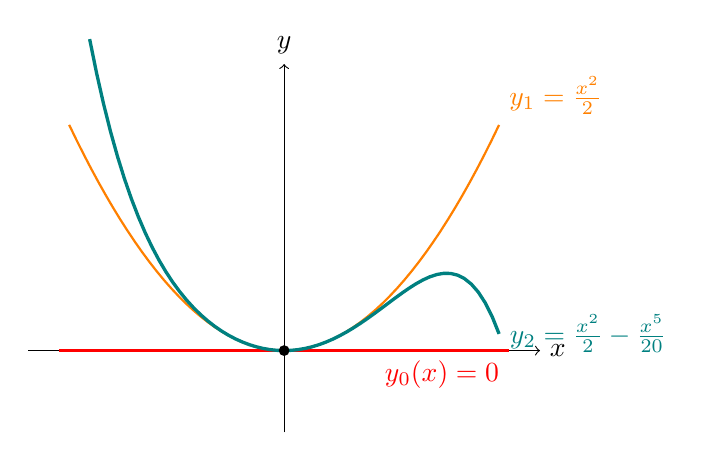
\begin{tikzpicture}[scale=1.3]
        % Оси координат
        \draw[->] (-2.5, 0) -- (2.5, 0) node[right] {$x$};
        \draw[->] (0, -0.8) -- (0, 2.8) node[above] {$y$};

        % y_0 = 0
        \draw[red, thick] (-2.2, 0) -- (2.2, 0)
            node[below left] {$y_0(x) = 0$};

        % y_1 = x^2 / 2
        \draw[orange, thick, domain=-2.1:2.1, samples=60]
            plot (\x, {0.5*\x*\x}) node[above right] {$y_1 = \frac{x^2}{2}$};

        % y_2 = x^2 / 2 - x^5 / 20
        \draw[teal, very thick, domain=-1.9:2.1, samples=60]
            plot (\x, {0.5*\x*\x - (\x*\x*\x*\x*\x)/20})
            node[right] {$y_2 = \frac{x^2}{2} - \frac{x^5}{20}$};

        % Начальная точка
        \fill[black] (0, 0) circle (1.5pt);
    \end{tikzpicture}
    \caption{Графики последовательных приближений Пикара $y_0, y_1, y_2$ для
    задачи Ф.221(а).}
\end{figure}

\begin{problem}[Ф.221(б)]
    Построить последовательные приближения Пикара $y_0, y_1, y_2$ для задачи
    Коши:
    \[
        \begin{cases}
            y' = y^2 + 3x^2 - 1, \\
            y(1) = 1.
        \end{cases}
    \]
\end{problem}

\begin{proof}[Решение]~\\
    \begin{quote}
        Здесь $f(x, y) = y^2 + 3x^2 - 1$, начальные данные: $x_0 = 1, y_0 = 1$.
        Вычисляем приближения по формуле \eqref{eq:l3_picard_seq}:
        \begin{enumerate}
            \item Нулевое приближение: $y_0(x) \equiv 1$.
            \item Первое приближение:
            \[
                y_1(x) = 1 + \int_{1}^{x} \left(1^2 + 3s^2 - 1\right) ds =
                1 + \int_{1}^{x} 3s^2 \, ds = 1 + \left. s^3 \right|_{1}^{x} = x^3.
            \]
            \item Второе приближение:
            \begin{align*}
                y_2(x) &= 1 + \int_{1}^{x} \left((s^3)^2 + 3s^2 - 1\right) ds =
                1 + \int_{1}^{x} \left(s^6 + 3s^2 - 1\right) ds \\
                &= 1 + \left. \left(\frac{s^7}{7} + s^3 - s\right) \right|_{1}^{x}
                = \frac{x^7}{7} + x^3 - x + \frac{6}{7}.
            \end{align*}
        \end{enumerate}
    \end{quote}
\end{proof}

\begin{figure}[H]
    \centering
    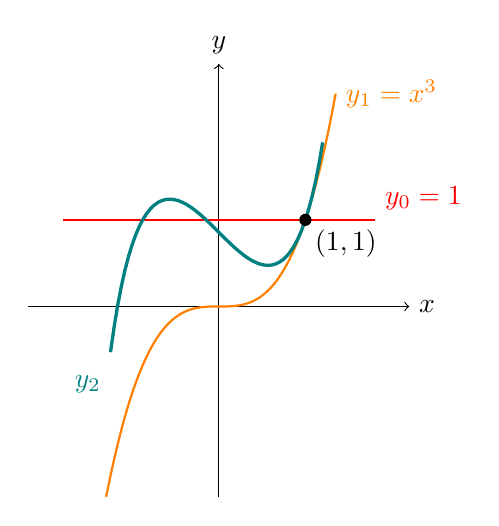
\begin{tikzpicture}[scale=1.1]
        % Оси координат
        \draw[->] (-2.2, 0) -- (2.2, 0) node[right] {$x$};
        \draw[->] (0, -2.2) -- (0, 2.8) node[above] {$y$};

        % y_0 = 1
        \draw[red, thick] (-1.8, 1) -- (1.8, 1) node[above right] {$y_0 = 1$};

        % y_1 = x^3
        \draw[orange, thick, domain=-1.3:1.35, samples=60]
            plot (\x, {\x*\x*\x}) node[right] {$y_1 = x^3$};

        % y_2 = x^7/7 + x^3 - x + 6/7
        \draw[teal, very thick, domain=-1.25:1.2, samples=60]
            plot (\x, {(\x*\x*\x*\x*\x*\x*\x)/7 + \x*\x*\x - \x + 6/7});
        \node[teal, left] at (-1.25, -0.9) {$y_2$};

        % Начальная точка
        \fill[black] (1, 1) circle (2pt) node[below right] {$(1, 1)$};
    \end{tikzpicture}
    \caption{Графики последовательных приближений Пикара $y_0, y_1, y_2$ для
    задачи Ф.221(б).}
\end{figure}

\begin{problem}[Ф.223(а)]
    Указать какой-нибудь отрезок, на котором гарантированно существует
    единственное решение задачи Коши:
    \[
        \begin{cases}
            y' = x + y^3, \\
            y(0) = 0.
        \end{cases}
    \]
\end{problem}

\begin{proof}[Решение]~\\
    \begin{quote}
        Правая часть $f(x, y) = x + y^3 \in C^\infty(\R^2)$, поэтому условия
        теоремы Пикара выполнены в любом замкнутом прямоугольнике $\Pi$ с
        центром в начальной точке $(x_0, y_0) = (0, 0)$:
        \[
            \Pi = \left\{ (x, y) \in \R^2 : \abs{x} \le a, \;
            \abs{y} \le b \right\}, \quad a, b > 0.
        \]
        Оценим максимум модуля функции $f(x, y)$ в $\Pi$:
        \[
            M = \max_{(x, y) \in \Pi} \abs{x + y^3} \le
            \max_{(x, y) \in \Pi} \left(\abs{x} + \abs{y}^3\right) = a + b^3.
        \]
        Тогда полудлина отрезка существования и единственности равна
        \[
            h = \min\left(a, \frac{b}{M}\right) =
            \min\left(a, \frac{b}{a + b^3}\right).
        \]
        Выберем параметры прямоугольника $a = 1, b = 1$. Подставляя их,
        получаем:
        \[
            h = \min\left(1, \frac{1}{1 + 1^3}\right) =
            \min\left(1, \frac{1}{2}\right) = \frac{1}{2}.
        \]
        Следовательно, решение задачи Коши существует и единственно на отрезке
        $[-1/2, 1/2]$.

        \textbf{Ответ:} $[-1/2, 1/2]$.
    \end{quote}
\end{proof}